%\documentclass[a4paper,10pt]{jarticle}
%\documentclass[]{jarticle}
\documentclass[10pt]{jarticle}

%\usepackage{graphicx}
\usepackage[dvipdfmx]{graphicx}
\usepackage{eclbkbox} %breakbox用

\usepackage{listings,jlisting}
%listingsの設定
\renewcommand{\lstlistingname}{ソースコード}
\lstset{language=sh,
  breaklines = true 
  basicstyle=\ttfamily\scriptsize,
  commentstyle=\textit,
  classoffset=1,
  showstringspaces=false
  keywordstyle=\bfseries,
  frame=tRBl,
  framesep=5pt,
  showstringspaces=false,
  numbers=left,
  stepnumber=1,
  numberstyle=\tiny,
  tabsize=2
}
%本文領域を広め(空白箇所マージン領域を小さめ)に設定
\setlength{\textwidth}{179mm}
\setlength{\textheight}{251mm}
\setlength{\topmargin}{-2cm}
\setlength{\oddsidemargin}{-1cm}
\setlength{\evensidemargin}{-1cm}

\begin{document}

\title{情報工学実験IIレポート(探索アルゴリズム2)}
\author{曜日&グループ番号: 月&グループ0} %
\date{2011年12月23日}

\maketitle

\begin{abstract}
このレポート(ファイル)は、「情報工学実験II・探索アルゴリズムその
2\cite{info2-search2}」の実験レポートの骨組みを例示している。
あくまでも例示であって、全てをこの通りに従う必要はないが、
指示された項目を含めた上で、
報告書として他者が読みやすいレポートとなるように工夫する事。
\end{abstract}

\section*{グループメンバ}
(補足:レベル毎に \underline{全員が協力して実施} した上で、レベル毎にレポートをまとめる担当者を決め、全体を一つのレポートとして整理すること。)
\begin{itemize}
 \item 945734J 當間愛晃: 担当Level1.1, 1.2, 3.4
 \item 945700 hoge: 担当Level2.1, 2,2, 3.5
 \item 945700 hoge: 担当Level3.1, 3.3
 \item 945700 hoge: 担当Level3.2
\end{itemize}

\section*{提出したレポート一式について}
レポート一式は
\verb|``naha:/home/home/teacher/tnal/jikken1-fri/e945734/''|
にアップロードした。
提出したファイルのディレクトリ構成は以下の通りである。\\
(補足:必ず下記のように整理しろという指定ではない。
自分たちでやりやすいようにLevel毎に整理しても構わない)
\begin{breakbox}
\begin{verbatim}
./src/      # 作成したプログラム一式
./report/   # レポート関係ファイル.図ファイルを含む.
\end{verbatim}
\end{breakbox}

\newpage

\section{Level1: 線形分離可能なOR問題への適用}
\subsection{課題説明}
2入力1出力で構成される単純パーセプトロン(ニューラルネットワーク)を
用いて、
4つの教師信号を用意したOR問題へ適用し、
重みが適切に学習可能であることを確認する。
また、学習が収束する様子をグラフとして示す。

 %課題説明
\subsection{OR問題を学習させた際の誤差収束度合いについて}
\subsubsection{実験結果}
NNでは重みを更新する毎に誤差が減るように学習を行うが、
その学習の様子は初期の重みをどのように設定したか、
学習に用いたパラメータをどのように設定したか、
といった対象問題以外の要素に影響して学習の様子が変化する。
シード値を変えた際の学習収束回数を表\ref{table:level1}に示す。
シード値を10回変更して学習させた際の重みを更新する様子を図
\ref{fig:level1-1}に、
その平均をプロットした平均推移値を図\ref{fig:level1-2}に示す。
なお、平均値を求める際には**して**した。
具体的には云々。

\begin{table}[htb]
 \begin{center}
  \caption{OR問題の学習に要した回数}
  \label{table:level1}
  \begin{tabular}[htb]{r|l} \hline
   シード値 & 収束した回数 \\ \hline \hline
   100 & hoge \\ \hline
   200 & hoge \\ \hline
   300 & hoge \\ \hline
   400 & hoge \\ \hline
   500 & hoge \\ \hline
   600 & hoge \\ \hline
   700 & hoge \\ \hline
   800 & hoge \\ \hline
   900 & hoge \\ \hline
   1000 & hoge \\ \hline \hline
   10試行の平均値 & hoge \\ \hline
  \end{tabular}
 \end{center}
\end{table}


\begin{figure}[h]
 \begin{center}
  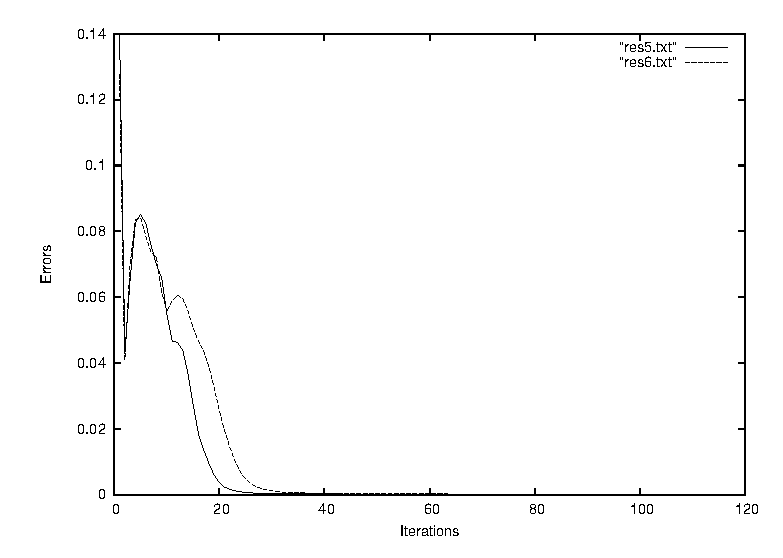
\includegraphics[width=10.0cm]{figs/sample1.eps}
  \caption{重みを更新する様子}
  \label{fig:level1-1}
 \end{center}
\end{figure}

\begin{figure}[h]
 \begin{center}
  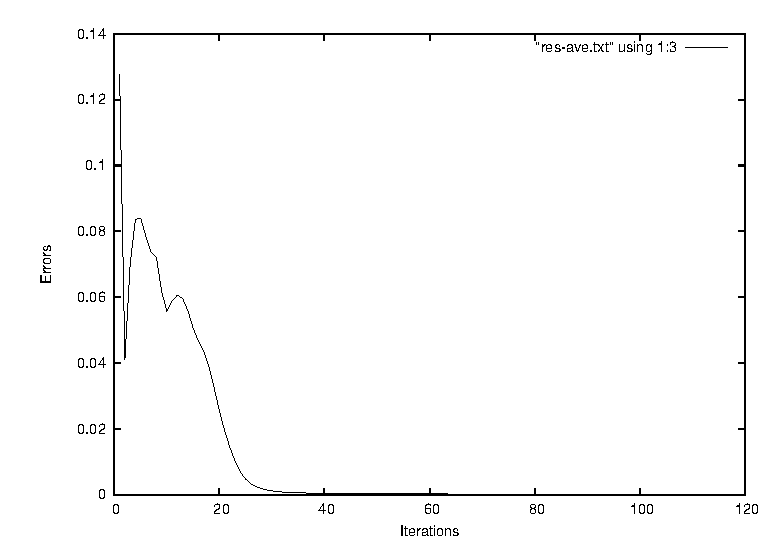
\includegraphics[width=10.0cm]{figs/sample2.eps}
  \caption{重みを更新する様子(平均値)}
  \label{fig:level1-2}
 \end{center}
\end{figure}


\subsubsection{考察}
(結果から分かったことは?)




\newpage

\section{Level2: 線形分離不可能なExOR問題への適用}
\subsection{課題説明}
階層型ニューラルネットワークをExOR問題へ適用し、
線形分離できない問題においても学習可能であることを確認する。
特にLevel2では、
この問題を解決するために中間層を導入することで拡張した階層型ニューラルネッ
トワークにより学習可能であることを確認する。



 %共通部分の結果及び考察
\subsection{$B3,AX7?(BNN$B$K$h$k3X=,(B}
\subsubsection{$B:GE,$J%Q%i%a!<%?$rC5$9$?$a$N%"%W%m!<%A(B}
$B;XDj$5$l$?>r7o2<$K$*$$$F3X=,$,8zN(NI$/9T$o$l$k%Q%i%a!<%?$NAH$_9g$o$;$rC5(B
$B$9$?$a!":G=i$O#1$D$NCM$E$D!"Bg$^$+$JCM$+$i@_Dj$7$FD4$Y!"=y!9$KCM$N:Y$+$/$7$F$$$/$3$H$G%Q%i%a!<%?$rD4@0$7$?!#(B\\
$B%Q%i%a!<%?$O0J2<$G$"$k!#(B\\
ETA:1.8643 \\
ALPHA:0.89 \\
HIDDEN:16 \\
$BJ?6Q<}B+2s?t(B:75.8\\
\subsubsection{$B%Q%i%a!<%?$NLO:wJ}K!(B}
$B%Q%i%a!<%?!<$O0J2<$N$h$&$K$7$F!"<B:]$KCM$rF~$l$F$_$F!"7k2L$r8+$J$,$i7hDj$7$?!#(B\\
$B8m:9$N$_$r8+$k$N$G$O$J$/!"%-%A%s$H<}B+$9$k$+$I$&$+$bD4$Y$J$,$iLO:w$7$?!#(B\\
\begin{itemize}
\item alpha n :::$B2s?t(B,$B8m:9(B
 \item alpha 0.1 :::394,0.0000997313
 \item alpha 0.5 :::17,0.0000998573
 \item alpha 0.8 :::87,0.0000938422
 \item alpha 0.89 :::48,0.0000934068
 \item alpha 0.90 :::44,0.0000820184
 \item alpha 0.94 :::32,0.0000489520
\end{itemize}
$B$3$N$h$&$J7k2L$K$J$C$?$,!"(Balpha=0.89$B0J>e$NCM$O<}B+$9$k2s?t$,A}$($F$$$/$?$a!"(Balpha=0.89$B$,%Y%9%H$@$H9M$($?!#(B\\
\subsubsection{$B<B9T7k2L(B}

\begin{table}[htb]
 \begin{center}
  \caption{$B3,AX7?(BNN$B$K$h$k(BExOR$BLdBj$N3X=,$KMW$7$?2s?t(B}
  \label{table:level2}
  \begin{tabular}[htb]{r|l} \hline
   $B%7!<%ICM(B & $B<}B+$7$?2s?t(B \\ \hline \hline
   1000 &  48\\ \hline
   2000 &  68\\ \hline
   3000 &  243\\ \hline
   4000 &  64\\ \hline
   5000 &  67\\ \hline
   6000 &  69\\ \hline
   7000 &  54\\ \hline
   8000 &  38\\ \hline
   9000 &  55\\ \hline
   10000 &  52\\ \hline \hline
   10$B;n9T$NJ?6Q<}B+2s?t(B &  75.8\\ \hline
  \end{tabular}
 \end{center}
\end{table}

\begin{figure}[h]
 \begin{center}
  \includegraphics[width=10.0cm]{figs/exor_ave.eps}
  \caption{$B=E$_$r99?7$9$kMM;R!JJ?6QCM!K(B}
  \label{fig:level2}
 \end{center}
\end{figure}


\subsubsection{$B9M;!(B}
alpha$B$d(BETA$B$O9b$$CM$NJ}$,8m:9$,Dc$$7k2L$H$J$C$?$,!"(BHIDDEN$B$K4X$7$F$OI,$:$7$b$=$&$G$O$J$/!"(B16$B$H$$$&Hf3SE*Dc$$?t;z$G8m:9$,>.$5$/$J$C$?$N$G!"Cf4VAX$N%f%K%C%H$OB?$1$l$PB?$$DxNI$$$H$$$&$o$1$G$O$J$$$H9M$($i$l$k!#(B


\newpage

\section{Level3: 応用事例:文字認識問題への適用}
\subsection{課題説明}
階層型NNを文字認識に適用し、考察する。
特に、用意された教師データと認識のしやすさに関する関係性や、
学習最適化のためのパラメータのチューニングおよび、
より柔軟性の高い認識方法に関する検討を行う。

 %課題説明
\subsection{Level3.1: パラメータのチューニング}
\subsubsection{最適なパラメータを探すためのアプローチ}
最適なパラメータを探すために,3つのパラメータをそれぞれを探索するスクリプトを作成した.
\begin{itemize}
	\item HIDDEN.sh :HIDDENの値を1ずつ書き換えながら平均値を出力
	\item ALPHA.sh  :引数に「ALPHAの初期値」「ALPHAの刻み値」「ALPHAの最大値」を取り,連続的に実行する.
	\item ETA.sh    :ALPHA.shと同様にETAを小刻みに変更しながら実行を行う.
\end{itemize}

\subsubsection{実行結果}
\begin{itemize}
	\item HIDDEN
	\item ETA:
	\item ALPHA:
\end{itemize}<++>

\begin{table}[htb]
 \begin{center}
  \caption{階層型NNによる文字認識問題の学習に要した回数}
  \label{table:level3}
  \begin{tabular}[htb]{r|l} \hline
   シード値 & 収束した回数 \\ \hline \hline
   100 & hoge \\ \hline
   200 & hoge \\ \hline
   300 & hoge \\ \hline
   400 & hoge \\ \hline
   500 & hoge \\ \hline
   600 & hoge \\ \hline
   700 & hoge \\ \hline
   800 & hoge \\ \hline
   900 & hoge \\ \hline
   1000 & hoge \\ \hline \hline
   10試行の平均値 & hoge \\ \hline
  \end{tabular}
 \end{center}
\end{table}

\begin{figure}[h]
 \begin{center}
  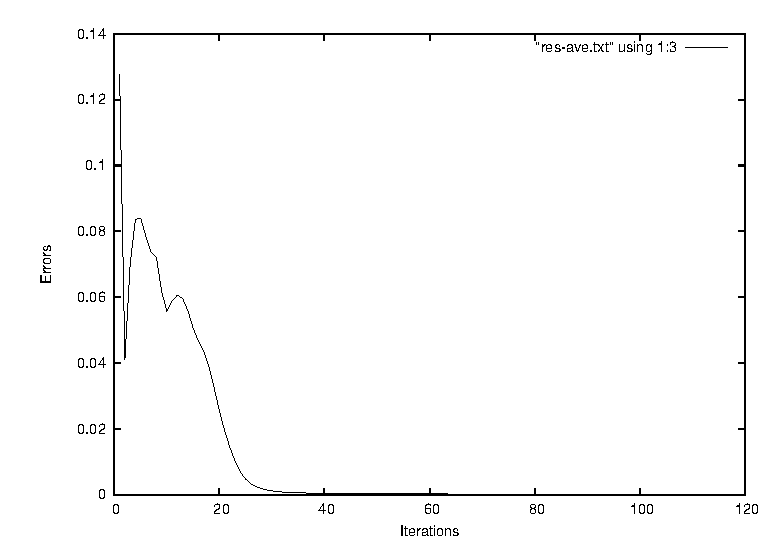
\includegraphics[width=10.0cm]{figs/sample2.eps}
  \caption{重みを更新する様子(平均値)}
  \label{fig:level2}
 \end{center}
\end{figure}


\subsubsection{考察}



\subsection{Level3.2: パラメータと収束能力の関連性について}
\subsubsection{関係性を確認するためのアプローチ}
3つのパラメータがどのような関係にあるかを検証するため、
ケース1,2,,,を設定し、学習曲線からその関係性について考察する。

\subsubsection{結果}

\subsubsection{考察}


\subsection{Level3.3: 任意の評価用データを用いた評価}
\subsubsection{アプローチ}

(仮説1)\\
学習時のデータ(教師データ)との違いが少ない程認識率が高く、
逆に教師データとの違いが多い程認識率が低くなるとの仮定の下、
明らかに見た目が違う評価データは用意せず教師データを拡大,位置移動,縮小
のような認識しやすい評価データと,認識しにくい斜めにした評価データを用意した。

\subsubsection{結果}

\begin{lstlisting}[caption=学習時のデータ拡大,label=ラベル]
nn> e
filename? --> data.num2/eva1-4.txt
correct = 0100000000
000111110000
000001000000
000001000000
000001000000
000001000000
000001000000
000001000000
000001000000
000001000000
000001000000
000001000000
000111110000
CHECK filename data.num2/eva1-4.txt
EVA o[0] = 0.03804, correct[0] = 0.1
EVA o[1] = 0.64843, correct[1] = 0.9
EVA o[2] = 0.18650, correct[2] = 0.1
EVA o[3] = 0.03347, correct[3] = 0.1
EVA o[4] = 0.16344, correct[4] = 0.1
EVA o[5] = 0.26652, correct[5] = 0.1
EVA o[6] = 0.06497, correct[6] = 0.1
EVA o[7] = 0.07104, correct[7] = 0.1
EVA o[8] = 0.07718, correct[8] = 0.1
EVA o[9] = 0.02484, correct[9] = 0.1
EVA sum_error = 0.85847
\end{lstlisting}


\begin{lstlisting}[caption=学習時のデータ位置移動,label=ラベル]
nn> e
filename? --> data.num2/eva1-5.txt
correct = 0100000000
000000000000
000000001110
000000000100
000000000100
000000000100
000000000100
000000000100
000000000100
000000000100
000000000100
000000001110
000000000000
CHECK filename data.num2/eva1-5.txt
EVA o[0] = 0.06909, correct[0] = 0.1
EVA o[1] = 0.13674, correct[1] = 0.9
EVA o[2] = 0.08040, correct[2] = 0.1
EVA o[3] = 0.44300, correct[3] = 0.1
EVA o[4] = 0.08931, correct[4] = 0.1
EVA o[5] = 0.30921, correct[5] = 0.1
EVA o[6] = 0.05398, correct[6] = 0.1
EVA o[7] = 0.04762, correct[7] = 0.1
EVA o[8] = 0.12550, correct[8] = 0.1
EVA o[9] = 0.24100, correct[9] = 0.1
EVA sum_error = 1.64158
\end{lstlisting}


\begin{lstlisting}[caption=学習時のデータ斜め,label=ラベル]
filename? --> data.num2/eva1-6.txt    
correct = 0100000000
000000000000
000000100000
000000001000
000000100010
000001000000
010010000000
000100000000
000010000000
000000000000
000000000000
000000000000
000000000000
CHECK filename data.num2/eva1-6.txt
EVA o[0] = 0.13168, correct[0] = 0.1
EVA o[1] = 0.22826, correct[1] = 0.9
EVA o[2] = 0.35467, correct[2] = 0.1
EVA o[3] = 0.14085, correct[3] = 0.1
EVA o[4] = 0.06984, correct[4] = 0.1
EVA o[5] = 0.17521, correct[5] = 0.1
EVA o[6] = 0.00947, correct[6] = 0.1
EVA o[7] = 0.34620, correct[7] = 0.1
EVA o[8] = 0.21842, correct[8] = 0.1
EVA o[9] = 0.15081, correct[9] = 0.1
EVA sum_error = 1.61026
\end{lstlisting}

\begin{lstlisting}[caption=学習時のデータ縮小,label=ラベル]
nn> e
filename? --> data.num2/eva1-7.txt 
correct = 0100000000
000000000000
000000000000
000011100000
000001000000
000001000000
000001000000
000001000000
000001000000
000001000000
000011100000
000000000000
000000000000
CHECK filename data.num2/eva1-7.txt
EVA o[0] = 0.08543, correct[0] = 0.1
EVA o[1] = 0.73866, correct[1] = 0.9
EVA o[2] = 0.08469, correct[2] = 0.1
EVA o[3] = 0.04289, correct[3] = 0.1
EVA o[4] = 0.14736, correct[4] = 0.1
EVA o[5] = 0.14030, correct[5] = 0.1
EVA o[6] = 0.03224, correct[6] = 0.1
EVA o[7] = 0.19359, correct[7] = 0.1
EVA o[8] = 0.07265, correct[8] = 0.1
EVA o[9] = 0.10494, correct[9] = 0.1
EVA sum_error = 0.52962
\end{lstlisting}

\subsubsection{考察}
Iを拡大,縮小,斜め,位置移動をしたものを評価用データとして認識テストを行った結果より,
拡大,縮小はほかのと比べエラーが低めだが,斜めそして予想に反して学習時のデータを平行移動させただけのデータでは
エラーがとても高くIとしては到底認識できていないことが分かった.
これよりこの文字の認識には学習時のデータの形はもちろんだがそれよりも位置が非常に重要になっていると予想できる.
\subsection{Level3.4: 認識率を高める工夫}
\subsubsection{対象とする問題点}
入力されたデータが想定していた入力と比べてサイズが異なったり、位置がずれている等、文字の一部が欠けている以外にも多様な要因によるデータ(情報)の劣化による認識率の低下.
\subsubsection{改善方法の提案}
	\begin{itemize}
	\item 学習時のデータをより多く様々な可能性を考え用意することで認識率を高める.
	\item 逆に認識したいデータとは全く違うデータを学習させ,認識率が低い場合に認識したいデータと判断する方法.
	\end{itemize}
\subsubsection{考察}
一つ目の提案では,例えばIを認識したいとき,斜め,拡大,縮小,位置変更をしたIをそれぞれ
複数学習させることにより,その学習時のデータの組み合わせにより様々な形のデータにも
認識率を高めることができると考えた.
二つ目の提案は,認識率が高いことにこだわらず逆に認識率が低いことに着眼点をおくことにより,逆転の発想でデータの認識率を高めることができると考えた.

\newpage
\section{その他: 実験の内容・進め方に関するコメント等}
(補足:
今後の為に参考にしたいので、情報工学実験2・探索アルゴリズム1,2で扱った
内容、実験の進め方等について意見があれば書いてください(当然、どのような
意見であってもレポートの評価を下げる事はしません。)。「授業評価アンケー
ト」の際に書いてもらっても構いません。)


\vspace{+1.0cm}
(補足:参考文献は thebibliography 環境を使って列挙し、
本文中で適切な箇所で引用するようにしましょう。
例えば下記文献は、アブストラクト中で引用しています)
\begin{thebibliography}{99}
\bibitem{info2-search2}
情報工学実験2: 探索アルゴリズムその2(當間)\\
\verb|http://www.eva.ie.u-ryukyu.ac.jp/~tnal/2011/info2/search2/|
\end{thebibliography}

\end{document}
